\documentclass[tikz, border=5mm]{standalone}
\usepackage{tikz}
\usetikzlibrary{shapes.geometric, arrows.meta, positioning, decorations.pathmorphing}

\begin{document}
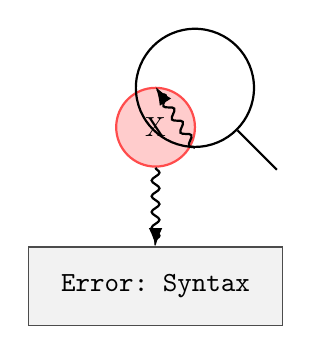
\begin{tikzpicture}[
    bug/.style={circle, draw=red!70, fill=red!20, thick, minimum size=1cm, inner sep=0pt},
    magnifying_glass/.style={
        draw, thick, circle, minimum size=1.5cm,
        append after command={
            \pgfextra{
                \draw[thick] (\tikzlastnode.south east) -- ++(0.5,-0.5);
            }
        }
    },
    error_text/.style={rectangle, draw=black!70, fill=gray!10, text width=3cm, text centered, minimum height=1cm, font=\ttfamily}
]

% Bug icon
\node (bug_node) at (0,0) [bug] {X}; % Placeholder for a bug icon

% Magnifying glass
\node (magnify_node) at (0.5,0.5) [magnifying_glass] {};

% Error message
\node (error_node) [error_text, below=1cm of bug_node] {Error: Syntax};

% Connection
\draw [decorate,decoration={snake,amplitude=.5mm,segment length=2mm}, -Latex, thick] (magnify_node.south) -- (bug_node.north);
\draw [decorate,decoration={snake,amplitude=.5mm,segment length=2mm}, -Latex, thick] (bug_node.south) -- (error_node.north);

\end{tikzpicture}
\end{document}